\documentclass{article}%
\usepackage[T1]{fontenc}%
\usepackage[utf8]{inputenc}%
\usepackage{lmodern}%
\usepackage{textcomp}%
\usepackage{lastpage}%
\usepackage{geometry}%
\geometry{top=3cm,bottom=2cm,left=2cm,right=2cm}%
\usepackage{float}%
\usepackage{ragged2e}%
\usepackage{tikz}%
%
%
%
\begin{document}%
\normalsize%
\section{Stack Operations}%
\label{sec:StackOperations}%

        \section*{Introduction}
        In programming and computer science, Stack is one of the important data structures that operate as a "last in, first out" (LIFO) structure. In other words, the last element added to the stack is the first element removed.
        %
\vspace{1cm}%
\begin{center}%
\begin{tabular}{cccc}%
\begin{minipage}[5.0pt]{0.2\textwidth}%
\centering%
\centering%
\vspace{1cm}%
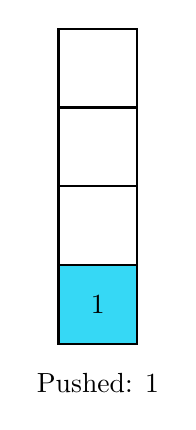
\begin{tikzpicture}%
\fill[fill={rgb,255:red,54;green,216;blue,245}] (0, 0.000000) rectangle (1.000000, 1.000000);%
\node[font=\fontsize{10.000000}{12.000000}\selectfont] at (0.500000, 0.500000) {1};%
\draw[thick] (0, 0) rectangle (1.000000, 4.000000);%
\draw[thick] (0, 1.000000) -- (1.000000, 1.000000);%
\draw[thick] (0, 2.000000) -- (1.000000, 2.000000);%
\draw[thick] (0, 3.000000) -- (1.000000, 3.000000);%
\node[font=\fontsize{10.000000}{12.000000}\selectfont] at (0.500000, -0.5) {Pushed: 1};%
\end{tikzpicture}%
\end{minipage}%
 & %
\begin{minipage}[5.0pt]{0.2\textwidth}%
\centering%
\centering%
\vspace{1cm}%
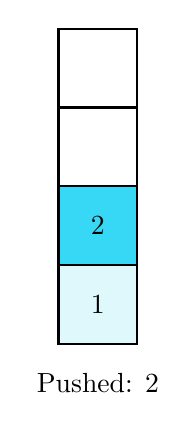
\begin{tikzpicture}%
\fill[fill={rgb,255:red,222;green,248;blue,252}] (0, 0.000000) rectangle (1.000000, 1.000000);%
\node[font=\fontsize{10.000000}{12.000000}\selectfont] at (0.500000, 0.500000) {1};%
\fill[fill={rgb,255:red,54;green,216;blue,245}] (0, 1.000000) rectangle (1.000000, 2.000000);%
\node[font=\fontsize{10.000000}{12.000000}\selectfont] at (0.500000, 1.500000) {2};%
\draw[thick] (0, 0) rectangle (1.000000, 4.000000);%
\draw[thick] (0, 1.000000) -- (1.000000, 1.000000);%
\draw[thick] (0, 2.000000) -- (1.000000, 2.000000);%
\draw[thick] (0, 3.000000) -- (1.000000, 3.000000);%
\node[font=\fontsize{10.000000}{12.000000}\selectfont] at (0.500000, -0.5) {Pushed: 2};%
\end{tikzpicture}%
\end{minipage}%
 & %
\begin{minipage}[5.0pt]{0.2\textwidth}%
\centering%
\centering%
\vspace{1cm}%
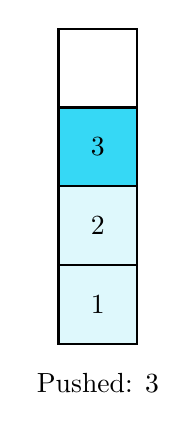
\begin{tikzpicture}%
\fill[fill={rgb,255:red,222;green,248;blue,252}] (0, 0.000000) rectangle (1.000000, 1.000000);%
\node[font=\fontsize{10.000000}{12.000000}\selectfont] at (0.500000, 0.500000) {1};%
\fill[fill={rgb,255:red,222;green,248;blue,252}] (0, 1.000000) rectangle (1.000000, 2.000000);%
\node[font=\fontsize{10.000000}{12.000000}\selectfont] at (0.500000, 1.500000) {2};%
\fill[fill={rgb,255:red,54;green,216;blue,245}] (0, 2.000000) rectangle (1.000000, 3.000000);%
\node[font=\fontsize{10.000000}{12.000000}\selectfont] at (0.500000, 2.500000) {3};%
\draw[thick] (0, 0) rectangle (1.000000, 4.000000);%
\draw[thick] (0, 1.000000) -- (1.000000, 1.000000);%
\draw[thick] (0, 2.000000) -- (1.000000, 2.000000);%
\draw[thick] (0, 3.000000) -- (1.000000, 3.000000);%
\node[font=\fontsize{10.000000}{12.000000}\selectfont] at (0.500000, -0.5) {Pushed: 3};%
\end{tikzpicture}%
\end{minipage}%
 & %
\begin{minipage}[5.0pt]{0.2\textwidth}%
\centering%
\centering%
\vspace{1cm}%
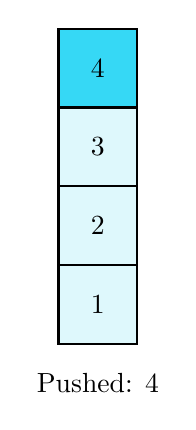
\begin{tikzpicture}%
\fill[fill={rgb,255:red,222;green,248;blue,252}] (0, 0.000000) rectangle (1.000000, 1.000000);%
\node[font=\fontsize{10.000000}{12.000000}\selectfont] at (0.500000, 0.500000) {1};%
\fill[fill={rgb,255:red,222;green,248;blue,252}] (0, 1.000000) rectangle (1.000000, 2.000000);%
\node[font=\fontsize{10.000000}{12.000000}\selectfont] at (0.500000, 1.500000) {2};%
\fill[fill={rgb,255:red,222;green,248;blue,252}] (0, 2.000000) rectangle (1.000000, 3.000000);%
\node[font=\fontsize{10.000000}{12.000000}\selectfont] at (0.500000, 2.500000) {3};%
\fill[fill={rgb,255:red,54;green,216;blue,245}] (0, 3.000000) rectangle (1.000000, 4.000000);%
\node[font=\fontsize{10.000000}{12.000000}\selectfont] at (0.500000, 3.500000) {4};%
\draw[thick] (0, 0) rectangle (1.000000, 4.000000);%
\draw[thick] (0, 1.000000) -- (1.000000, 1.000000);%
\draw[thick] (0, 2.000000) -- (1.000000, 2.000000);%
\draw[thick] (0, 3.000000) -- (1.000000, 3.000000);%
\node[font=\fontsize{10.000000}{12.000000}\selectfont] at (0.500000, -0.5) {Pushed: 4};%
\end{tikzpicture}%
\end{minipage}%
\\[2ex]%
\vspace{1cm}%
\end{tabular}%
\end{center}%
\vspace{2cm}%
\begin{center}%
\begin{tabular}{cccc}%
\begin{minipage}[5.0pt]{0.2\textwidth}%
\centering%
\centering%
\vspace{1cm}%
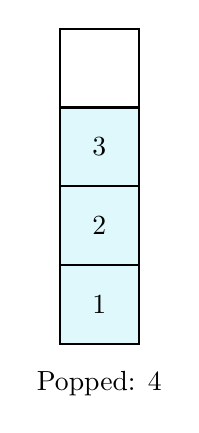
\begin{tikzpicture}%
\fill[fill={rgb,255:red,222;green,248;blue,252}] (0, 0.000000) rectangle (1.000000, 1.000000);%
\node[font=\fontsize{10.000000}{12.000000}\selectfont] at (0.500000, 0.500000) {1};%
\fill[fill={rgb,255:red,222;green,248;blue,252}] (0, 1.000000) rectangle (1.000000, 2.000000);%
\node[font=\fontsize{10.000000}{12.000000}\selectfont] at (0.500000, 1.500000) {2};%
\fill[fill={rgb,255:red,222;green,248;blue,252}] (0, 2.000000) rectangle (1.000000, 3.000000);%
\node[font=\fontsize{10.000000}{12.000000}\selectfont] at (0.500000, 2.500000) {3};%
\draw[thick] (0, 0) rectangle (1.000000, 4.000000);%
\draw[thick] (0, 1.000000) -- (1.000000, 1.000000);%
\draw[thick] (0, 2.000000) -- (1.000000, 2.000000);%
\draw[thick] (0, 3.000000) -- (1.000000, 3.000000);%
\node[font=\fontsize{10.000000}{12.000000}\selectfont] at (0.500000, -0.5) {Popped: 4};%
\end{tikzpicture}%
\end{minipage}%
 & %
\begin{minipage}[5.0pt]{0.2\textwidth}%
\centering%
\centering%
\vspace{1cm}%
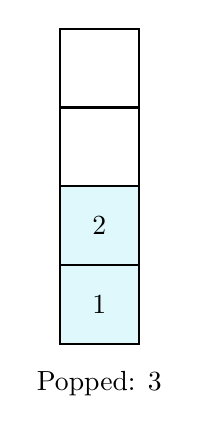
\begin{tikzpicture}%
\fill[fill={rgb,255:red,222;green,248;blue,252}] (0, 0.000000) rectangle (1.000000, 1.000000);%
\node[font=\fontsize{10.000000}{12.000000}\selectfont] at (0.500000, 0.500000) {1};%
\fill[fill={rgb,255:red,222;green,248;blue,252}] (0, 1.000000) rectangle (1.000000, 2.000000);%
\node[font=\fontsize{10.000000}{12.000000}\selectfont] at (0.500000, 1.500000) {2};%
\draw[thick] (0, 0) rectangle (1.000000, 4.000000);%
\draw[thick] (0, 1.000000) -- (1.000000, 1.000000);%
\draw[thick] (0, 2.000000) -- (1.000000, 2.000000);%
\draw[thick] (0, 3.000000) -- (1.000000, 3.000000);%
\node[font=\fontsize{10.000000}{12.000000}\selectfont] at (0.500000, -0.5) {Popped: 3};%
\end{tikzpicture}%
\end{minipage}%
 & %
\begin{minipage}[5.0pt]{0.2\textwidth}%
\centering%
\centering%
\vspace{1cm}%
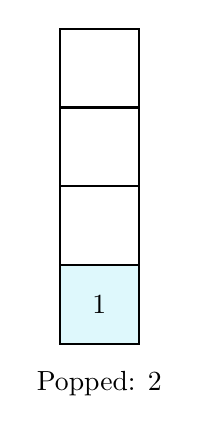
\begin{tikzpicture}%
\fill[fill={rgb,255:red,222;green,248;blue,252}] (0, 0.000000) rectangle (1.000000, 1.000000);%
\node[font=\fontsize{10.000000}{12.000000}\selectfont] at (0.500000, 0.500000) {1};%
\draw[thick] (0, 0) rectangle (1.000000, 4.000000);%
\draw[thick] (0, 1.000000) -- (1.000000, 1.000000);%
\draw[thick] (0, 2.000000) -- (1.000000, 2.000000);%
\draw[thick] (0, 3.000000) -- (1.000000, 3.000000);%
\node[font=\fontsize{10.000000}{12.000000}\selectfont] at (0.500000, -0.5) {Popped: 2};%
\end{tikzpicture}%
\end{minipage}%
 & %
\begin{minipage}[5.0pt]{0.2\textwidth}%
\centering%
\centering%
\vspace{1cm}%
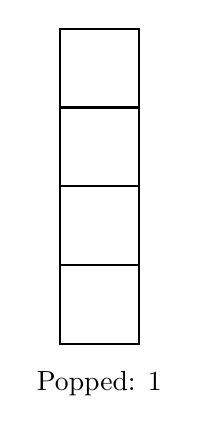
\begin{tikzpicture}%
\draw[thick] (0, 0) rectangle (1.000000, 4.000000);%
\draw[thick] (0, 1.000000) -- (1.000000, 1.000000);%
\draw[thick] (0, 2.000000) -- (1.000000, 2.000000);%
\draw[thick] (0, 3.000000) -- (1.000000, 3.000000);%
\node[font=\fontsize{10.000000}{12.000000}\selectfont] at (0.500000, -0.5) {Popped: 1};%
\end{tikzpicture}%
\end{minipage}%
\\[2ex]%
\vspace{1cm}%
\end{tabular}%
\end{center}

%
\end{document}